%\documentclass{standalone}
%\usepackage{tikz}
%
%\begin{document}

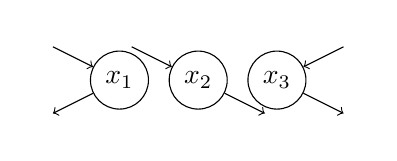
\begin{tikzpicture}
\node at (-1, 0.5) [shape=circle] (in1) {};
\node at (-1, -0.5) [shape=circle] (out1) {};
\node at (0, 0) [shape=circle, draw] (x1) {$x_1$};
\node at (1, 0) [shape=circle, draw] (x2) {$x_2$};
\node at (2, 0) [shape=circle, draw] (x3) {$x_3$};
\node at (0, 0.5) [shape=circle] (in2) {};
\node at (2, -0.5) [shape=circle] (out2) {};
\node at (3, 0.5) [shape=circle] (in3) {};
\node at (3, -0.5) [shape=circle] (out3) {};
\draw [->] (in1) to  (x1);
\draw [->] (x1) to (out1);
\draw [->] (in2) to (x2);
\draw [->] (x2) to (out2);
\draw [->] (in3) to (x3);
\draw [->] (x3) to (out3);
\end{tikzpicture}

%\end{document}
